
\documentclass[preprint,12pt]{elsarticle}

\usepackage[spanish]{babel}
\usepackage{amssymb}
\usepackage{graphicx}
\usepackage{lineno}
\usepackage[utf8]{inputenc}
\usepackage{url}
\usepackage{natbib}

\begin{document}
	
	\begin{frontmatter}

		\title{\huge  DEVOPS EN LA BASE DE DATOS}
		
		\author{Robles Flores, Anthony Richard	              (2016056192)}
		\author{Porlles Carrillo, Diego Armando              (2015050948)}
		\author{Sandoval Blas, Jesus Enrique           (2016054467)}
		\author{Quispe Mamani, José Luis              (2015053235)}
		
		\address{Tacna, Perú}
		
		\begin{abstract}
%%ANTHONYROBLES*******************************************************************************************************************
			%% Text of abstract
DevOps is a conceptual framework for reintegrating development and operations of Information Systems. We performed a Systematic Mapping Study to explore DevOps. 26 articles out of 139 were selected, studied and summarized. Based on this a concept table was constructed. We discov-ered that DevOps has not been adequately studied in scientific literature. There is relatively little research available on DevOps and the studies are often of low quality. 
\\
\\
We also found that DevOps is supported by a culture of collaboration, automation, measurement, information sharing and web service usage. DevOps benefits IS development and operations performance. It also has positive effects on web service development and quality assurance performance. Finally, our mapping study suggests that more research is needed to quantify these effects.
		\end{abstract}
\end{frontmatter}
%%
	%% Start line numbering here if you want
	%%
	%\linenumbers
	
	%% main text
	\section{Resumen}

DevOps es un marco conceptual para reintegrar el desarrollo y las operaciones de los sistemas de información. Realizamos un estudio de mapeo sistemático para explorar DevOps. 26 artículos de 139 fueron seleccionados, estudiados y resumidos. En base a esto, se construyó una tabla conceptual. Descubrimos que DevOps no se ha estudiado adecuadamente en la literatura científica. Hay relativamente poca investigación disponible sobre DevOps y los estudios a menudo son de baja calidad. 
\\
\\
También descubrimos que DevOps está respaldado por una cultura de colaboración, automatización, medición, intercambio de información y uso de servicios web. DevOps beneficia el desarrollo de IS y el rendimiento de las operaciones. También tiene efectos positivos en el desarrollo del servicio web y el rendimiento del aseguramiento de la calidad. Finalmente, nuestro estudio de mapeo sugiere que se necesita más investigación para cuantificar estos efectos.
%%https://www.researchgate.net/publication/267330992_Report_DevOps_Literature_Review



%%INTRODUCCION%%-------------------------------------------------------------------------------------------
\section{Introducción}
El desarrollo ágil divide en iteraciones el desarrollo de un sistema software para
obtener incrementos de software funcional. A pesar de los beneficios del desarrollo
ágil, se originan nuevos retos debido a las brechas que aparecen al momento de integrar, realizar pruebas y desplegar a producción cada incremento. Además, el tiempo
de entrega de cada incremento es un factor importante que origina una ventaja competitiva a las organizaciones, permitiendo obtener retroalimentación de los clientes y de
esta manera realizar una mejora continua de los productos de software.
Realizar manualmente los procesos de integración, pruebas y despliegue de incrementos de software ocasiona en la mayoría de los casos retrasos en la planificación de
los proyectos y es propenso a errores con un resultado no confiable
\\
\\
DevOps es un
conjunto de principios y prácticas que optimizan el tiempo de entrega de software,
gestionan la infraestructura como código y mejoran la experiencia del usuario en base
a la retroalimentación de sus comentarios. Las prácticas de DevOps  son:
 i) la integración continua construye todo el software y ejecuta un conjunto de pruebas con
cada incremento, ii) el despliegue continuo toma el software creado en la integración
y lo despliega en un entorno de operaciones de una manera automática, y iii) la entrega continua proporciona la capacidad de liberar en el entorno de operaciones nuevas
versiones de software varias veces al día.
\\
\\
Es un método de reconfiguración dinámica incremental de arquitecturas
de servicios cloud basado en el Desarrollo de Software Dirigido por Modelos
(DSDM). Este método tiene como objetivo apoyar a los desarrolladores de software
en la integración incremental de servicios en entornos cloud, por tal motivo provee un
conjunto de actividades que soportan: i) el diseño de la integración, ii) la implementación de la integración, y iii) el despliegue y reconfiguración arquitectónica.
%%-------------------------------------------------------------------------------------------

%MARCO TEORICO-------------------------------------------------------------------------------------------
\section{Marco Teórico}

\subsection{Definición}

DevOps es una metodología de desarrollo de software que apunta a reunir equipos de desarrollo de software y operativos de tecnología de la información. Es un concepto que fomenta una cultura de colaboración entre estos dos equipos que históricamente trabajaron en sus propios silos separados, desde la fase de diseño inicial hasta el lanzamiento del producto.

DevOps es una metodología que combina el desarrollo de software (Dev) con las operaciones (Ops). La intención es permitir la comunicación entre los equipos para que puedan construir, probar y lanzar software más rápidamente y con mayor eficiencia y velocidad.

Al combinar estos dos equipos y procesos distintos, se promueve la integración continua, la implementación continua, las pruebas automatizadas y la transparencia en los repositorios de código.


\cite{DWarehouse02}
\\
\\

\begin{figure}[htb]
				\begin{center}
					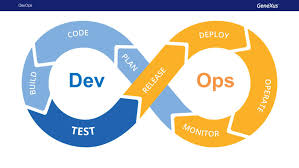
\includegraphics[width=9cm]{./IMAGENES/definicionsql}
				\end{center}
			\end{figure}

\subsection{¿Qué es Agile?}
La metodología ágil es también una metodología de desarrollo de software que surgió alrededor del año 2001, cuando se presentó el manifiesto ágil. Emplea cuatro valores y doce principios que ayudan a construir una cultura de desarrollo de software "ágil".

En términos generales, ágil fomenta la adopción y una mentalidad de liderazgo que promueve el trabajo en equipo, la autoorganización y la responsabilidad. Más importante aún, el enfoque ágil se enfoca más en alinear continuamente el desarrollo con las necesidades y tendencias del cliente, incluso cuando esas necesidades y tendencias cambian al final del proceso de desarrollo.
\\
\\
Agile incorpora un conjunto de principios que ayudan a individuos, equipos y unidades más grandes a trabajar juntos. La "mentalidad ágil" se enfoca más en las personas que en los procesos y herramientas. Una organización ágil se adapta y aprende sobre el cambio constante que les permite identificar nuevas oportunidades y añadir más valor para los clientes. "SQL-92" o "SQL2".\cite{DWarehouse02}
\\
\\

\begin{figure}[htb]
				\begin{center}
					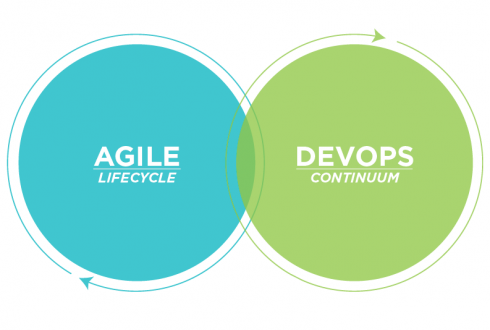
\includegraphics[width=10.5cm]{./IMAGENES/evolucion}
				\end{center}
			\end{figure}


\subsection{Requisitos para implementar una cultura DevOps}
Lo primero es comunicar que la cultura DevOps se va a implementar, mencionando los beneficios y haciendo que el equipo se sienta parte del cambio. Luego explicar las acciones que se van a tomar, no importa que no sean desarrolladores.

La comunicación y colaboración para tener una cultura DevOps son cruciales, es un trabajo entre los desarrolladores y los equipos encargados de la infraestructura de los servidores.

La tarea principal será la automatización, reducir los tiempos de despliegue del producto y mantener una calidad de desarrollo y estabilidad para el usuario. Debes tener claro que esto será un proceso sin fin, por lo que cada mejora te dará el tiempo que dedicarás para innovar el proceso y hacerlo cada vez mejor.
%%S*******************************************************************************************************************

%%JOSE LUIS*******************************************************************************************************************
\subsection{Contradicciones en DevOps de base de datos}
Como podemos ver, las bases de datos se ha vuelto una parte muy importante en el proceso de modernización de las aplicaciones, lo cual puede presentar un problema intratable.

En DevOps para entornos de prueba de bases de datos, las organizaciones deben generar rápidamente clones del sistema para ofrecer datos que reflejen con precisión el entorno de producción, al tiempo que protegen la información corporativa sensible. Por otro lado, los cambios de la base de datos en la producción representan el abismo más amplio entre las técnicas de desarrollo de aplicaciones ágil y la capacidad de desplegarlas en infraestructuras de TI del mundo real.\cite{DLake01}

\subsection{DevOps de base de datos desafía los problemas de pruebas}
Normalmente, los desarrolladores son los primeros en descubrir las dificultades técnicas de trabajar con bases de datos en entornos de prueba automatizados.
"No tienen los datos correctos", dijo Brandon Cipes, director gerente de DevOps en cPrime, una firma de consultoría ágil en Foster City, California. "¿Cómo hacen que el entorno de prueba ilustre la producción, y cómo mantienen ese ambiente actualizado y seguro?".
Las herramientas de gestión de datos de prueba están disponibles de proveedores como DBmaestro y CA Technologies, pero es aquí donde empiezan a surgir desafíos de personas y procesos, dijo Nirmal Mehta, tecnólogo jefe de la firma de consultoría Booz Allen Hamilton.

\subsection{Las bases de datos de producción presentan desafíos adicionales de DevOps}
Para abordar estos problemas, algunas organizaciones han movido las aplicaciones de producción a bases de datos NoSQL, que no requieren esquemas. 
Sin embargo, muchos han retrocedido después de que los sistemas NoSQL presentaran problemas de gestión en la producción, dijo Cook.
"Muchos equipos se dieron cuenta de que, cuando la gente decía que MongoDB era más simple, significaba para la instalación", dijo Cook.
\\
 "Pero para una aplicación de producción, la gente termina por tener que construir un esquema y un sistema de sanitización de datos encima de todos modos, y si no eres un DBA [administrador de bases de datos], NoSQL se convierte en un desastre muy fácilmente".
"De repente, Postgres se convirtió en el mejor de ambos mundos", dijo Cook.
Según Rob Steward, vicepresidente de desarrollo de producto de Progress Software, “una buena práctica de DevOps liberará a los desarrolladores para que se centren en hacer lo que mejor saben hacer: escribir software. DevOps elimina el trabajo y las preocupaciones de la puesta en producción del software una vez que está escrito”.

%%*******************************************************************************************************************

\section{Analisis}
\subsection{DevOps en entorno de pruebas de Bases de Datos}
DevOps para el entorno de prueba de Base de Datos más que solución podrían ocasionar problemas en el entorno con referencia al uso de Contenedores y el tema del precio
\\
Según el siguiente Párrafo.
\\
"Extraer los datos de producción de una cola y clonar el tráfico de producción para obtener insumos realistas puede ocasionar costos de infraestructura que muchas organizaciones no quieren pagar", dijo Nirmal Mehta, tecnólogo jefe de la firma de consultoría Booz Allen Hamilton.
\\

Los contenedores son el furor en las pruebas de aplicaciones automatizadas porque los desarrolladores pueden crearlos rápidamente y luego destruirlos, pero las aplicaciones de base de datos con estado aún no se prestan bien a la contenerización.

"Hasta cierto punto, hay una incongruencia fundamental entre las bases de datos y los contenedores", dijo E.T. Cook, principal defensor de la firma de consultoría etc.io, que ayuda a las empresas a desplegar contenedores. 
\\
Si bien hay herramientas que te permiten el almacenamiento persistente en aplicaciones contenerizadas, pero los enfoques más probados no resuelven el problema de la verdadera portabilidad de datos, dijo Cook.

Existen productos que ofrecen un almacenamiento persistente de contenedores verdaderamente distribuido, pero las empresas todavía deben aprender cómo administrar e integrar estos sistemas.

A pesar de la disponibilidad de estas herramientas, muchas empresas aún desarrollan sus propias capas de abstracción para administrar múltiples tipos de bases de datos. Estas capas de abstracción actúan como amortiguadores entre las aplicaciones y las bases de datos, para que los cambios en cualquiera de ellos no interrumpan al otro, dijo Cipes de cPrime.

\textbf{''Las bases de datos de producción presentan desafíos adicionales de DevOps''}

Incluso cuando los problemas de DevOps en bases de datos se resuelven en la prueba, el abismo sigue siendo amplio entre el entorno de prueba y la infraestructura de producción donde se ejecutarán realmente las aplicaciones. Las bases de datos de producción pueden ser engorrosas para actualizar, requieren el conocimiento tribal de esquemas de datos complejos para acceder y operar, y son lentas para escalar. Pero también las Bases de datos Avanzan con el pasar del tiempo incorporando objetos no esquemáticos, que permiten que los datos no estructurados sean parte de las consultas contra índices y con el tiempo de seguro los problemas que existían anteriormente cada vez se volverá tan pequeño que el uso de devOps ya no será un impedimento para que las empresas decidan usarlo , siendo uno de las metodologías mas favoritas que hay en la actualidad ofreciendo Resultado Tangibles y adoptado por las organizaciones un Total de 1425 según la información en 2014. Devops: Salir victoriosos en la economía de las aplicaciones


%%-------------------------------------------------------------------------------------------


%CONCLUSIONES-------------------------------------------------------------------------------------------
\section{Conclusiones}
%%JOSE LUIS***************************************************************************************************************************************
\subsection{Conclusión }	
En conclusión, sacaremos una definición simple de DevOps con la que podamos estar de acuerdo, y este concepto es que DevOps es una metodología de desarrollo de software basada en la integración entre desarrolladores de software basada en la integración entre desarrolladores y administradores de sistemas, que permite que los desarrolladores puedan enfocarse solo en desarrollar y puedan desplegar su código en segundos.
%%***************************************************************************************************************************************

%%-------------------------------------------------------------------------------------------

%%
	
	%%
	%\linenumbers
	
	%% main text

	
	\newpage
	
	\bibliographystyle{apalike} 	%ESTILO
	\bibliography{BIBLIOGRAFIA}	 
\citep{DLake01}  
\citep{DLake02}  
\citep{DWarehouse01}  
\citep{DWarehouse02}   
	

\end{document}

